\begin{flushright} {\tiny {\color{gray} coordinate\_systems.tex}} \end{flushright}
%~~~~~~~~~~~~~~~~~~~~~~~~~~~~~~~~~~~~~~~~~~~~~~~~~~~~~~~~~~~~~~~~~~~~~~~~~~~~~~~~~~~~~~~~~~~~~~~~~~

\begin{center}
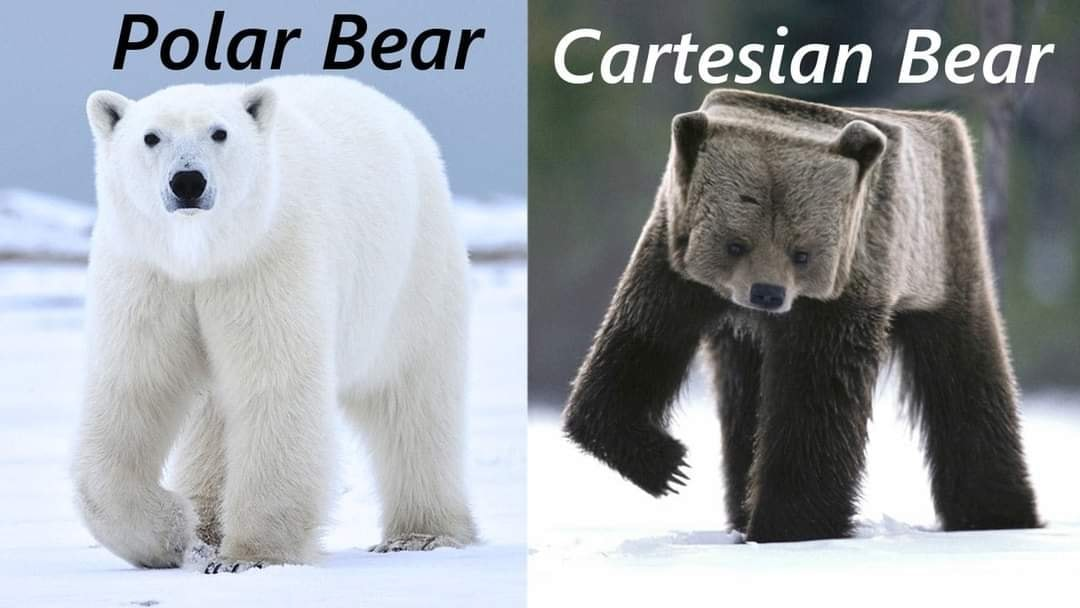
\includegraphics[width=6cm]{images/polarbear}
\end{center}

%........................................
\subsubsection{Cartesian coordinates}
\index{general}{Gradient Operator in Cartesian Coordinates}
\index{general}{Divergence Operator in Cartesian Coordinates}
\index{general}{Laplace Operator in Cartesian Coordinates}
\index{general}{Path Increment in Cartesian Coordinates}

The unit vectors along the $x$, $y$ and $z$ axis are 
$\vec{e}_x$, $\vec{e}_y$ and $\vec{e}_z$ respectively.

\begin{flushright} {\tiny {\color{gray} (tikz\_cartesian\_coordinates.tex)}} \end{flushright}
%~~~~~~~~~~~~~~~~~~~~~~~~~~~~~~~~~~~~~~~~~~~~~~~~~~~~~~~~~~~~~~~~~~~~~~~~~~~~~~~~~~~~~~~~~~~~~~~~~~
\begin{center}
\begin{tikzpicture}
%\draw[step=0.5cm,gray,very thin] (0,0) grid (4,4); %background grid

\draw [thick,->] (1.5,2) -- (3.5,2);
\draw [thick,->] (1.5,2) -- (1.5,4);
\draw [thick,->] (1.5,2) -- (0.5,0.5);

\node[] at (0.75,0.25) {$x$};
\node[] at (3.75,2) {$y$};
\node[] at (1.75,3.75) {$z$};

\draw[>=triangle 45, line width=0.3mm, ->] (1.5,2) -- (2.5,2) ;   
\node[] at (2,1.7) {$\vec{e}_x$};

\draw[>=triangle 45, line width=0.3mm, ->] (1.5,2) -- (1.5,3) ;   
\node[] at (1.9,2.75) {$\vec{e}_y$};

\draw[>=triangle 45, line width=0.3mm, ->] (1.5,2) -- (1,1.25) ;   
\node[] at (1.25,1.1) {$\vec{e}_z$};

\end{tikzpicture}
\end{center}


\noindent Any vector can then be written
\[
{\vec V}  = V_x {\vec e}_x  + V_y {\vec e}_y + V_z \vec{e}_z
\]
'How much of $\vec{V}$ is there in the $x-$direction' is obtained
with $\vec{V}\cdot\vec{e}_x = V_x$.
The gradient of a function $f$ is 
\[
\vec{\nabla} f= \text{grad }f= 
\frac{\partial f}{\partial x}\; \vec{e}_x +
\frac{\partial f}{\partial y}\; \vec{e}_y +
\frac{\partial f}{\partial z}\; \vec{e}_z,
\]
the divergence of a vector $\vec{V}$ is
\[
\vec{\nabla}\cdot \vec{V} = 
\frac{\partial V_x}{\partial x}+
\frac{\partial V_y}{\partial y}+
\frac{\partial V_z}{\partial z}
\]
and the Laplace operator of a function $f$ is:
\[
\Delta f = 
\frac{\partial^2 f}{\partial x^2} + 
\frac{\partial^2 f}{\partial y^2} + 
\frac{\partial^2 f}{\partial z^2}  
\]
Finally the path increment is
\[
d\vec{r} = dx \; {\vec e}_x  + dy\; {\vec e}_y + dz \; \vec{e}_z
\]
and the volume element is 
\[
dV=dx\; dy \; dz.
\]

%........................................
\subsubsection{Polar coordinates}

We have $r>0$ and $\theta=[0,2\pi[$, defined in the $(x,y)-$plane.

\begin{flushright} {\tiny {\color{gray} (tikz\_polar\_coordinates.tex)}} \end{flushright}
%~~~~~~~~~~~~~~~~~~~~~~~~~~~~~~~~~~~~~~~~~~~~~~~~~~~~~~~~~~~~~~~~~~~~~~~~~~~~~~~~~~~~~~~~~~~~~~~~~~
\begin{center}
\begin{tikzpicture}
%\draw[step=0.5cm,gray,very thin] (0,0) grid (4.5,4); %background grid

\draw [thick,->] (1,1) -- (3.5,1);
\draw [thick,->] (1,1) -- (1,3.5);

\node[] at (3.5,0.75) {$x$};
\node[] at (0.6,3.5) {$y$};

\draw[>=triangle 45, line width=0.3mm, ->] (1,1) -- (2,1) ;   
\node[] at (1.6,0.75) {$\vec{e}_x$};

\draw[>=triangle 45, line width=0.3mm, ->] (1,1) -- (1,2) ;   
\node[] at (0.6,1.7) {$\vec{e}_y$};

\draw [-] (1,1) -- (3,2);

\draw[>=triangle 45, line width=0.3mm, ->] (3,2) -- (4,2.5) ;   
\node[] at (4.25,2.5) {$\vec{e}_r$};

\draw[>=triangle 45, line width=0.3mm, ->] (3,2) -- (2.5,3) ;   
\node[] at (2.5,3.25) {$\vec{e}_\theta$};


\node[] at (2.2,1.75) {$r$};
\node[] at (2.25,1.3) {$\theta$};

\draw[->] (2,1) arc (0:22.5:1.25);

\end{tikzpicture}
\end{center}


\noindent The relation between the unit vector in Cartesian and Polar/Cylindrical coordinates
is given by:
\[
\left(
\begin{array}{c}
{\vec e}_{r} \\
{\vec e}_{\theta} \\
\end{array}
\right)
=
\left(
\begin{array}{cc}
\cos \theta & \sin \theta \\
-\sin \theta & \cos \theta
\end{array}
\right)
\cdot
\left(
\begin{array}{c}
{\vec e}_{x} \\
{\vec e}_{y} \\
\end{array}
\right)
\]
which should be read:
\begin{eqnarray}
{\vec e}_{r}      &=& \cos\theta \; {\vec e}_{x} + \sin\theta \;  {\vec e}_{y} \nn\\
{\vec e}_{\theta} &=& -\sin\theta \; {\vec e}_{x} + \cos\theta \;  {\vec e}_{y} 
\end{eqnarray}
Obviously for $\theta=0$ we find $\vec{e}_r=\vec{e}_x$ and $\vec{e}_\theta = \vec{0}$, while for 
$\theta=\pi/2$ then $\vec{e}_r=\vec{0}$ and $\vec{e}_\theta=\vec{e}_y$.

Note that this $2\times 2$ matrix is a 
rotation matrix\footnote{\url{https://en.wikipedia.org/wiki/Rotation_matrix}}
corresponding to an angle $-\theta$. The inverse of this matrix always exists 
(we can always counter-rotate) and it then yields
\[
\left(
\begin{array}{c}
{\vec e}_{x} \\
{\vec e}_{y} \\
\end{array}
\right)
=
\left(
\begin{array}{cc}
\cos \theta & -\sin \theta \\
\sin \theta & \cos \theta
\end{array}
\right)
\cdot
\left(
\begin{array}{c}
{\vec e}_{r} \\
{\vec e}_{\theta} \\
\end{array}
\right)
\]
so that for any vector ${\vec V}$
\begin{eqnarray}
{\vec V} 
&=& V_x {\vec e}_x  + V_y {\vec e}_y \nonumber\\
&=& V_x [(\cos \theta) {\vec e}_r - (\sin \theta) {\vec e}_\theta]  + 
    V_y [(\sin \theta) {\vec e}_r + (\cos \theta){\vec e}_\theta] \nonumber\\
&=& [V_x (\cos \theta) + V_y (\sin \theta)] {\vec e}_r +
[- V_x(\sin \theta) + V_y (\cos \theta)]{\vec e}_\theta \nn\\
&=& V_r \vec{e}_r  + V_\theta \vec{e}_\theta \nn
\end{eqnarray}
with
\begin{eqnarray}
V_r &=& V_x \cos \theta + V_y \sin \theta \nn\\
V_\theta &=& - V_x \sin \theta + V_y \cos \theta \nn
\end{eqnarray}
Finally the path increment is
\[
d\vec{r} = dr \; {\vec e}_r  + r \sin\theta d\theta \; {\vec e}_\theta
\]
and the volume element is 
\[
dV= r dr \; d\theta.
\]
The gradient, divergence and Laplacian formulae are given in the following section about 
the cylindrical coordinates.

\index{general}{Path Increment in Polar Coordinates}

%...........................................................
\subsubsection{Cylindrical coordinates \label{ss:cylcoord}}

%Redo with tikz
\begin{center}
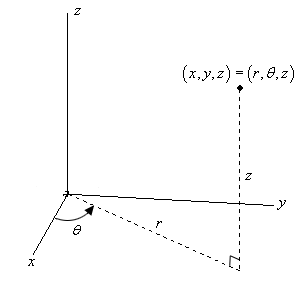
\includegraphics[width=4cm]{images/cylindrical}\\
{\captionfont Cylindrical coordinates}
%https://tutorial.math.lamar.edu/classes/calcii/CylindricalCoords.aspx 
\end{center}

\[
{\vec V} 
= V_r \; \vec{e}_r  + V_\theta \; \vec{e}_\theta + V_z \; \vec{e}_z
\]
We have 
\begin{eqnarray}
x &=& r \; \cos\theta \nn\\
y &=& r \; \sin \theta \nn\\\ 
r &=& \sqrt{x^2+y^2} \nn
\end{eqnarray}

Let $f(r,\theta)$ be a function of the spatial coordinates. Its gradient is then
\[
\vec \nabla f
= \frac{\partial f}{\partial r} \; \vec{e}_r 
+ \frac{1}{r} \frac{\partial f}{\partial \theta} \; \vec{e}_\theta
+ \frac{\partial f}{\partial r} \; \vec{e}_z
\]
The divergence of a vector field $\vec{V}$ is 
\[
\vec\nabla \cdot \vec{V} 
= \frac{1}{r} \frac{\partial }{\partial r} (r V_r) 
+ \frac{1}{r} \frac{\partial V_\theta}{\partial \theta} 
+ \frac{\partial V_z}{\partial z}
\]
and the Laplacian of $f$ is
\[
\Delta f = \frac{1}{r} \frac{\partial }{\partial r} \left( r \frac{\partial f}{\partial r} \right)
+ \frac{1}{r^2} \frac{\partial^2 f}{\partial \theta^2} 
+ \frac{\partial^2 f}{\partial z^2} 
\]
Finally the path increment is
\[
d\vec{r} = dr \; {\vec e}_r  + r \sin\theta d\theta \; {\vec e}_\theta + dz \; \vec{e}_z
\]
and the volume element is 
\[
dV= r dr \; d\theta \; dz
\]
\index{general}{Gradient Operator in Cylindrical Coordinates}
\index{general}{Divergence Operator in Cylindrical Coordinates}
\index{general}{Laplace Operator in Cylindrical Coordinates}
\index{general}{Path Increment in Cylindrical Coordinates}

\begin{remark} 
Cylindrical coordinates can also be denoted by $(\rho,\theta)$, $(r,\phi)$ or even $(\rho,\phi)$.
They are sometimes called "cylindrical polar coordinates" or "polar cylindrical coordinates".
\end{remark}

%........................................
\subsubsection{Spherical coordinates \label{ss:sphercoord}}

On the following figure are represented the three Cartesian axis, 
a point and its spherical coordinates $r,\theta,\phi$:
\begin{center}
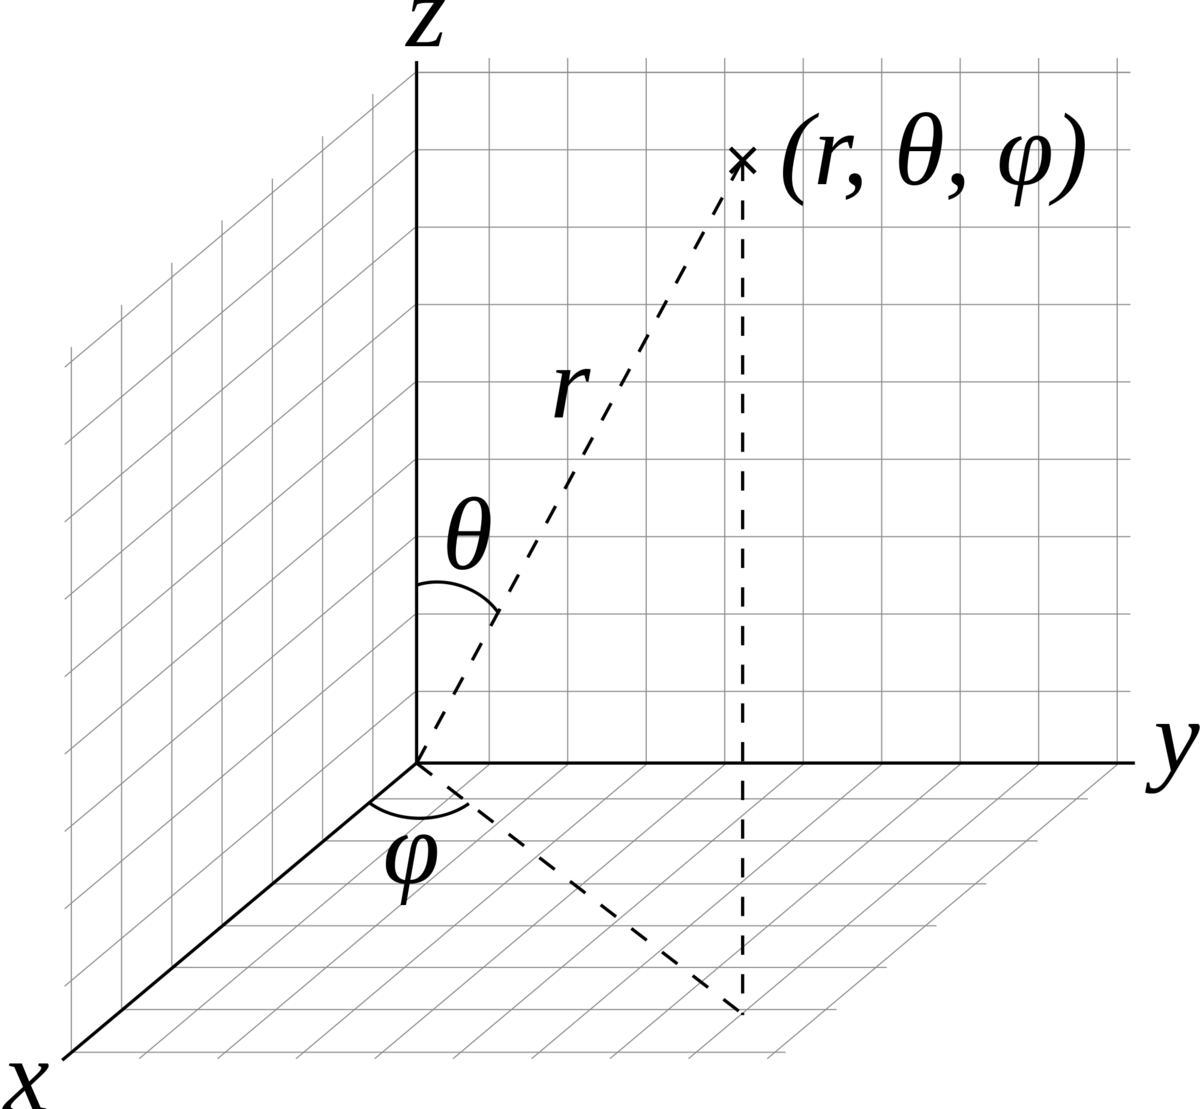
\includegraphics[width=5cm]{images/sphcoord}\\
{\captionfont Spherical coordinates as commonly used in physics:\\ polar angle $\theta$, and azimuthal angle $\phi$.} 
\end{center}
In this case $\theta\in[0:\pi]$ and $\phi\in]-\pi:\pi]$ and we have the following relationships:
\begin{eqnarray}
r &=& \sqrt{x^2+y^2+z^2} \\
\theta &=& \arccos (z/r) \\
\phi &=& \arctan (y/x) \\
x &=& r \sin \theta \cos \phi \\
y &=& r \sin\theta \sin\phi \\
z &=& r \cos\theta 
\end{eqnarray}
The inverse tangent used to compute $\phi$ must be suitably defined, 
taking into account the correct quadrant of $(x,y)$,
which is why the atan2 intrinsic function is used in \textsc{FORTRAN} for example.    
This is often written as follows:
\begin{eqnarray}
\theta &=& \arctan \left(\sqrt{x^2+y^2},z\right) \\
\phi &=& \arctan (y,x) 
\end{eqnarray}
where we formally take advantage of the two argument arctan
function to eliminate quadrant confusion.

The path increment is expressed as:

\begin{equation}
d\vec{r} = dr \; \vec{e}_r + r d\theta \; \vec{e}_\theta + r \sin\theta d\phi \; \vec{e}_\phi
\end{equation}
The gradient of a function $f(r,\theta,\phi)$ is 
\begin{equation}
\vec\nabla f= \frac{\partial f}{\partial r} \; \vec{e}_r
+ \frac{1}{r} \frac{\partial f}{\partial \theta} \; \vec{e}_\theta 
+ \frac{1}{r \; \sin\theta} \frac{\partial f}{\partial \phi} \;  \vec{e}_\phi
\end{equation}
The divergence of a vector $\vec{V}$ is
\begin{equation}
\vec\nabla\cdot \vec{V}=
\frac{1}{r^2} \frac{\partial}{\partial r} \left(r^2 V_r \right) 
+
\frac{1}{r \sin\theta} \frac{\partial}{\partial \theta} (V_\theta \sin\theta)
+
\frac{1}{r \sin\theta} \frac{\partial V_\phi}{\partial \phi}=0
\label{eq:divsc}
\end{equation}
The Laplacian of function $f$ is given by: \index{general}{Laplacian}
\begin{equation}
\Delta f= \vec\nabla \cdot\vec\nabla f= \vec\nabla^2 f
=
\frac{1}{r^2}\frac{\partial}{\partial r} \left( r^2 \frac{\partial f}{\partial r} \right)
+\frac{1}{r^2 \sin\theta} \frac{\partial}{\partial \theta} \left( \sin\theta \frac{\partial f}{\partial \theta} \right)
+\frac{1}{r^2 \sin^2\theta}  \frac{\partial^2 f}{\partial \phi^2}
\end{equation}

In geography one uses latitude and longitude, represented hereunder:
\begin{center}
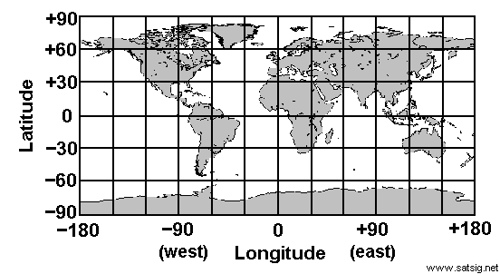
\includegraphics[width=10cm]{images/map.jpg}
\end{center}
\begin{itemize}
\item Latitude  $\in[-90:90]$,   or $\in[-\pi/2:\pi/2]$ 
\item Longitude $\in]-180:180]$, or $\in]-\pi:\pi]$ 
\end{itemize}

Since the colatitude is the complementary angle of the latitude, 
i.e. the difference between 90 and the latitude, 
where southern latitudes are denoted with a minus sign,
$\theta$ as shown above is actually is the colatitude.
The colatitude is shown in red on the following figure: 
\index{general}{Colatitude}
\begin{center}
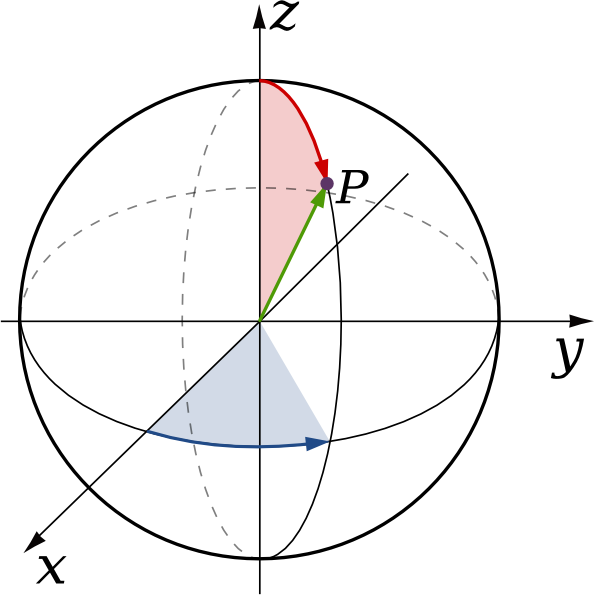
\includegraphics[width=3cm]{images/colatitude}
\end{center}

The volume of a sphere of radius $R$ is easily obtained by computing 
\begin{eqnarray}
V_{sphere} 
&=& \iiint_{sphere} dV \nn\\
&=& \int_0^R r^2 dr \int_0^\pi \sin\theta d\theta \int_0^{2\pi} d\phi  \nn\\
&=& \frac{1}{3}R^3  \cdot 2 \cdot 2\pi \nn\\
&=& \frac{4}{3}\pi R^3 
\end{eqnarray}
\index{general}{Volume of a Sphere}

The volume of a spherical shell of inner radius $R_i$ and outer radius $R_o$
is equally easily obtained by computing 

\begin{eqnarray}
V_{shell}
&=& \iiint_{shell} dV \nn\\
&=& \int_{R_i}^{R_o} r^2 dr \int_0^\pi \sin\theta d\theta \int_0^{2\pi} d\phi  \nn\\
&=& \frac{1}{3}(R_o^3-R_i^3)  \cdot 2 \cdot 2\pi \nn\\
&=& \frac{4}{3}\pi (R^3_o -R^3_i)
\end{eqnarray}
\index{general}{Volume of a Spherical shell}


\noindent The spherical unit vectors are related to the Cartesian unit vectors by:
\[
\left(
\begin{array}{c}
\vec{e}_{r} \\ \vec{e}_\theta \\ \vec{e}_\phi
\end{array}
\right)
=
\left(
\begin{array}{ccc}
\sin\theta \cos\phi & \sin\theta\sin\phi & \cos\theta  \\
\cos\theta \cos\phi & \cos\theta\sin\phi & -\sin\theta \\
-\sin\phi & \cos\phi & 0
\end{array}
\right)
\left(
\begin{array}{c}
\vec{e}_{x} \\ \vec{e}_y \\ \vec{e}_z
\end{array}
\right)
\]
and the Cartesian unit vectors are related to the spherical unit vectors by

\[
\left(
\begin{array}{c}
\vec{e}_{x} \\ \vec{e}_y \\ \vec{e}_z
\end{array}
\right)
=
\left(
\begin{array}{ccc}
\sin\theta \cos\phi & \cos\theta\cos\phi & -\sin\phi  \\
\sin\theta \sin\phi & \cos\theta\sin\phi & \cos\phi \\
\cos\theta & -\sin\theta & 0
\end{array}
\right)
\left(
\begin{array}{c}
\vec{e}_{r} \\ \vec{e}_\theta \\ \vec{e}_\phi
\end{array}
\right)
\]
Finally, the velocity vector $\vec{\upnu}$ then becomes
\begin{eqnarray}
\vec{\upnu} 
&=& u\; \vec{e}_x + v \; \vec{e}_y + w \; \vec{e}_z \nn\\
&=& u\; ( \sin\theta \cos\phi \; \vec{e}_r +  \cos\theta\cos\phi \;  \vec{e}_{\theta} -\sin\phi \; \vec{e}_{\phi} ) \nn\\
&+& v\; ( \sin\theta \sin\phi \; \vec{e}_r + \cos\theta\sin\phi \; \vec{e}_\theta  +  \cos\phi \;  \vec{e}_\phi  )  \nn\\
&+& w\; ( \cos\theta \; \vec{e}_r   -\sin\theta \; \vec{e}_\theta  ) \nn\\
&=& v_r\; \vec{e}_r + v_\theta\; \vec{e}_\theta + v_\phi\; \vec{e}_\phi 
\end{eqnarray}
with 
\begin{eqnarray}
v_r      &=&  u \sin \theta  \cos \phi  + v \sin\theta \sin \phi + w \cos\theta \\
v_\theta &=&  u \cos\theta\cos\phi + v \cos\theta\sin\phi -w \sin\theta   \\
v_\phi   &=& -u \sin\phi  + v \cos\phi  
\end{eqnarray}

%.................................................................................................
\subsubsection{Converting tensors between Cartesian and Cylindrical bases \label{ss:convcartspher}}

\[
{\bm T}_{\tiny Cyl}=
\left(
\begin{array}{ccc}
T_{rr}       & T_{r\theta}      & T_{rz} \\
T_{\theta r} & T_{\theta\theta} & T_{\theta z} \\
T_{z r}      & T_{z \theta}     & T_{zz}
\end{array}
\right)
=
\left(
\begin{array}{ccc}
 \cos \theta&\sin \theta&0 \\
-\sin \theta&\cos \theta&0 \\
0 & 0 & 1 
\end{array}
\right)
\cdot
\left(
\begin{array}{ccc}
T_{xx} & T_{xy} & T_{xz} \\
T_{yx} & T_{yy} & T_{yz} \\
T_{zx} & T_{zy} & T_{zz} 
\end{array}
\right)
\cdot
\left(
\begin{array}{ccc}
\cos \theta & -\sin \theta&0 \\
\sin \theta &  \cos \theta&0 \\
0 & 0 & 1 
\end{array}
\right)
\]

\[
{\bm T}_{\tiny Cart}=
\left(
\begin{array}{ccc}
T_{xx} & T_{xy} & T_{xz} \\
T_{yx} & T_{yy} & T_{yz} \\
T_{zx} & T_{zy} & T_{zz} 
\end{array}
\right)
=
\left(
\begin{array}{ccc}
 \cos \theta&-\sin \theta&0 \\
\sin \theta&\cos \theta&0 \\
0 & 0 & 1 
\end{array}
\right)
\cdot
\left(
\begin{array}{ccc}
T_{rr}       & T_{r\theta}      & T_{rz} \\
T_{\theta r} & T_{\theta\theta} & T_{\theta z} \\
T_{z r}      & T_{z \theta}     & T_{zz}
\end{array}
\right)
\cdot
\left(
\begin{array}{ccc}
\cos \theta & \sin \theta&0 \\
-\sin \theta &  \cos \theta&0 \\
0 & 0 & 1 
\end{array}
\right)
\]



%.................................................................................................
\subsubsection{Converting tensors between Cartesian and Spherical bases \label{ss:convcartspher}}

Let ${\bm T}$ be a tensor
\[
{\bm T}=
\left(
\begin{array}{ccc}
T_{xx} & T_{xy} & T_{xz} \\
T_{yx} & T_{yy} & T_{yz} \\
T_{zx} & T_{zy} & T_{zz} 
\end{array}
\right)
\qquad\qquad
{\bm T}=
\left(
\begin{array}{ccc}
T_{rr}       & T_{r\theta}      & T_{r\phi} \\
T_{\theta r} & T_{\theta\theta} & T_{\theta\phi} \\
T_{\phi r}   & T_{\phi \theta}  & T_{\phi\phi}
\end{array}
\right)
\]
in the Cartesian basis (left) and the spherical basis (right).

The two sets of components are related by
\[
\left(
\begin{array}{ccc}
T_{xx} & T_{xy} & T_{xz} \\
T_{yx} & T_{yy} & T_{yz} \\
T_{zx} & T_{zy} & T_{zz} 
\end{array}
\right)
=
\left(
\begin{array}{ccc}
\sin\theta \; \cos\phi & \cos\theta \; \cos\phi & -\sin\phi \\
\sin\theta \; \sin\phi & \cos\theta \; \sin\phi &  \cos\phi \\
\cos\theta & -\sin\theta & 0 
\end{array}
\right)
\cdot
\left(
\begin{array}{ccc}
T_{rr}       & T_{r\theta}      & T_{r\phi} \\
T_{\theta r} & T_{\theta\theta} & T_{\theta\phi} \\
T_{\phi r}   & T_{\phi \theta}  & T_{\phi\phi}
\end{array}
\right)
\cdot
\left(
\begin{array}{ccc}
\sin\theta\;\cos\phi & \sin\theta\;\sin\phi & \cos\theta \\
\cos\theta\;\cos\phi & \cos\theta\;\sin\phi & -\sin\theta \\
-\sin\phi & \cos\phi & 0 
\end{array}
\right)
\]
or
\[
\left(
\begin{array}{ccc}
T_{rr}       & T_{r\theta}      & T_{r\phi} \\
T_{\theta r} & T_{\theta\theta} & T_{\theta\phi} \\
T_{\phi r}   & T_{\phi \theta}  & T_{\phi\phi}
\end{array}
\right)
=
\left(
\begin{array}{ccc}
\sin\theta \; \cos\phi & \sin\theta \; \sin\phi & \cos\theta \\
\cos\theta \; \cos\phi & \cos\theta \; \sin\phi & -\sin\theta \\
-\sin\phi & \cos\phi & 0 
\end{array}
\right)
\cdot
\left(
\begin{array}{ccc}
T_{xx} & T_{xy} & T_{xz} \\
T_{yx} & T_{yy} & T_{yz} \\
T_{zx} & T_{zy} & T_{zz} 
\end{array}
\right)
\cdot
\left(
\begin{array}{ccc}
\sin\theta\;\cos\phi & \cos\theta\;\cos\phi & -\sin\phi \\
\sin\theta\;\sin\phi & \cos\theta\;\sin\phi & \cos\phi \\
\cos\theta & -\sin\theta & 0
\end{array}
\right)
\]
If we now assume that the tensor ${\bm T}$ is symmetric (e.g. stress tensor, strain rate tensor),
then there are only 6 independent terms.

